\documentclass{article}
\usepackage[utf8]{inputenc}
\usepackage[spanish]{babel}
\usepackage{amsmath}
\usepackage{graphicx}
\usepackage{booktabs}
\usepackage[margin=1in]{geometry}
\usepackage{float}

\title{Informe de Análisis de Escalabilidad de Random Forest}
\author{Análisis de Resultados de HPC}
\date{\today}

\begin{document}
\maketitle

\begin{abstract}
Este informe presenta un análisis de rendimiento y escalabilidad de un clasificador \textit{Random Forest} (Bosque Aleatorio) implementado con \texttt{scikit-learn} sobre un conjunto de datos sintéticos, variando el número de hilos de procesamiento ($P$) y el tamaño de la muestra ($N$). Los resultados demuestran una aceleración significativa en el tiempo de ajuste ($T_{\text{fit}}$) con el aumento de $P$, aunque con una eficiencia que disminuye progresivamente debido a la sobrecarga paralela. También se observa que el tiempo de ajuste escala de forma super-lineal con el tamaño de la muestra, lo cual es consistente con la complejidad algorítmica esperada. La exactitud del modelo se mantuvo alta y estable en todas las ejecuciones.
\end{abstract}

\section{Configuración del Experimento}

El experimento se ejecutó sobre una plataforma de Cómputo de Alto Rendimiento (HPC), utilizando el sistema de colas \texttt{SLURM} (script \texttt{rf.sh}). Se realizaron pruebas variando dos parámetros clave:

\begin{itemize}
    \item \textbf{Número de Hilos ($P$ o \texttt{n\_jobs})}: $P \in \{1, 2, 4, 8, 16, 32\}$.
    \item \textbf{Tamaño de la Muestra ($N$ o \texttt{n\_samples})}: $N \in \{100k, 200k, 400k, 800k\}$.
\end{itemize}

Todos los demás hiperparámetros del \textit{Random Forest} se mantuvieron fijos: \texttt{n\_estimators} $= 400$, \texttt{max\_depth} $= 20$, \texttt{n\_features} $= 40$. Los tiempos reportados son el promedio de $\text{reps}=3$ ejecuciones.

\section{Resultados Generales}

La \textbf{Tabla \ref{tab:rf_results}} resume los resultados clave, incluyendo la aceleración relativa ($S(P)$). La aceleración se calculó tomando como base el menor $P$ ejecutado para cada tamaño de muestra ($P_{\min}$), es decir, $S_{\text{rel}}(P) = T(P_{\min}) / T(P)$. Para $N=100k$, $P_{\min}=1$, lo que permite una comparación con la aceleración ideal.

\begin{table}[H]
\centering
\caption{Resultados de Escalabilidad del Clasificador Random Forest}
\label{tab:rf_results}
\begin{tabular}{cccccc}
\toprule
   P &      N &  $T_{\text{fit}}$ (s) &  $T_{\text{pred}}$ (s) &  Accuracy &  S(P) Relativo \\
\midrule
 $1$ & $100k$ &                274.37 &                 1.1016 &    0.9629 &           1.00 \\
 $2$ & $100k$ &                148.80 &                 0.6270 &    0.9629 &           1.84 \\
 $4$ & $100k$ &                 76.56 &                 0.3244 &    0.9629 &           3.58 \\
 $8$ & $100k$ &                 42.29 &                 0.1898 &    0.9629 &           6.49 \\
$16$ & $100k$ &                 24.64 &                 0.1223 &    0.9629 &          11.14 \\
$32$ & $100k$ &                 18.89 &                 0.1277 &    0.9629 &          14.53 \\
 $2$ & $200k$ &                326.52 &                 1.3565 &    0.9761 &           1.00 \\
 $4$ & $200k$ &                170.80 &                 0.6889 &    0.9761 &           1.91 \\
 $8$ & $200k$ &                 94.10 &                 0.3926 &    0.9761 &           3.47 \\
$16$ & $200k$ &                 54.53 &                 0.2398 &    0.9761 &           5.99 \\
$32$ & $200k$ &                 40.52 &                 0.1964 &    0.9761 &           8.06 \\
 $4$ & $400k$ &                373.66 &                 1.5633 &    0.9794 &           1.00 \\
 $8$ & $400k$ &                207.67 &                 0.8622 &    0.9794 &           1.80 \\
$16$ & $400k$ &                124.06 &                 0.5367 &    0.9794 &           3.01 \\
$32$ & $400k$ &                 90.23 &                 0.4911 &    0.9794 &           4.14 \\
 $8$ & $800k$ &                478.50 &                 1.8504 &    0.9814 &           1.00 \\
$16$ & $800k$ &                284.56 &                 1.1617 &    0.9814 &           1.68 \\
$32$ & $800k$ &                194.10 &                 1.0769 &    0.9814 &           2.47 \\
\bottomrule
\end{tabular}
\end{table}

\subsection{Exactitud del Modelo}
La exactitud (\textit{Accuracy}) fue consistentemente alta y estable para cada tamaño de muestra, variando entre $0.9629$ ($N=100k$) y $0.9814$ ($N=800k$). Esto indica que las variaciones en $P$ no afectaron la calidad del modelo entrenado.

\section{Análisis de Escalabilidad por Hilos ($P$)}

\begin{figure}[H]
    \centering
    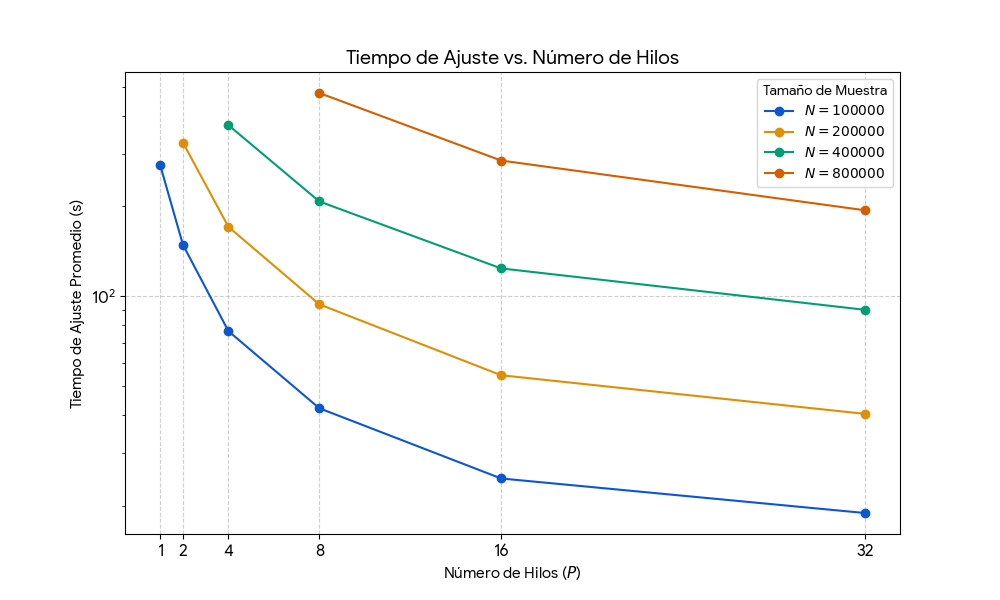
\includegraphics[width=0.8\textwidth]{fit_time_vs_n_samples_p32.png}
    \caption{Tiempo de Ajuste ($T_{\text{fit}}$) vs. Número de Hilos ($P$)}
    \label{fig:fit_time_vs_n_jobs}
\end{figure}

La \textbf{Figura \ref{fig:fit_time_vs_n_jobs}} muestra que el tiempo de ajuste disminuye significativamente a medida que se aumenta el número de hilos.

\begin{itemize}
    \item \textbf{Aceleración del Ajuste ($T_{\text{fit}}$)}: Para $N=100k$, el tiempo de ajuste se reduce de $274.37s$ ($P=1$) a $18.89s$ ($P=32$). Esto representa una aceleración de $S(32) \approx 14.53$ veces.
    \item \textbf{Eficiencia de Paralelización}: Como se muestra en la \textbf{Figura \ref{fig:speedup_vs_n_jobs}}, el caso $N=100k$ se mantiene cerca de la línea de aceleración ideal ($S=P$) hasta $P=8$. A partir de $P=16$ y $P=32$, la eficiencia del paralelismo se reduce, con una eficiencia de $\frac{14.53}{32} \approx 45.4\%$ en $P=32$. Esta caída se debe típicamente a la sobrecarga de comunicación y sincronización entre los hilos, que se vuelve dominante sobre la ganancia de paralelizar la construcción de los árboles.
\end{itemize}

\begin{figure}[H]
    \centering
    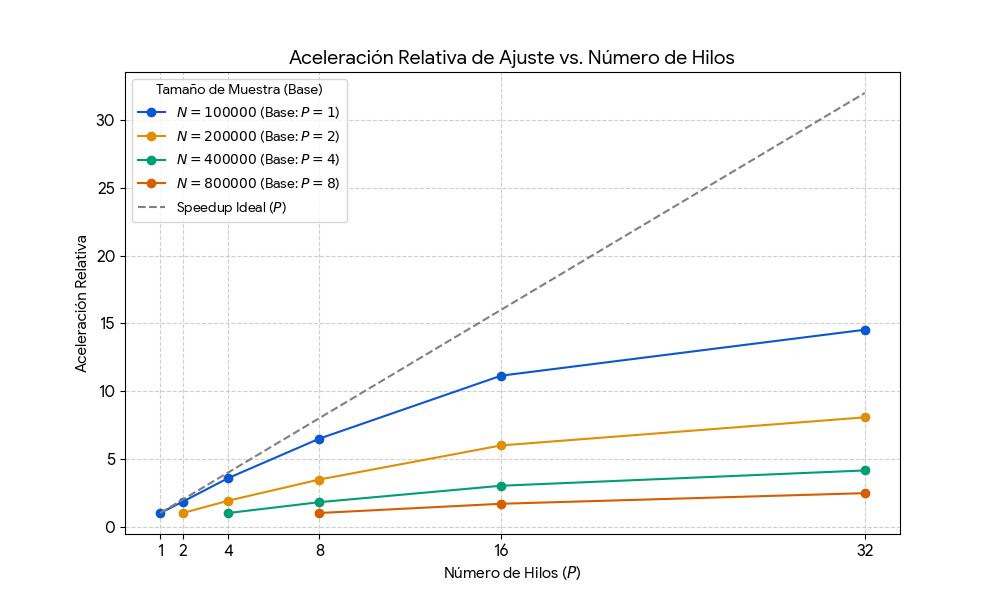
\includegraphics[width=0.8\textwidth]{speedup_vs_n_jobs.png}
    \caption{Aceleración Relativa ($S_{\text{rel}}(P)$) vs. Número de Hilos ($P$)}
    \label{fig:speedup_vs_n_jobs}
\end{figure}

\subsection{Tiempo de Predicción ($T_{\text{pred}}$)}
El tiempo de predicción también se beneficia del paralelismo, aunque la aceleración es menor que en el ajuste. Para $N=100k$, el tiempo se reduce de $1.1016s$ ($P=1$) a $0.1277s$ ($P=32$), logrando una aceleración de $\approx 8.63$ veces.

\section{Análisis de Complejidad por Tamaño de Muestra ($N$)}

\begin{figure}[H]
    \centering
    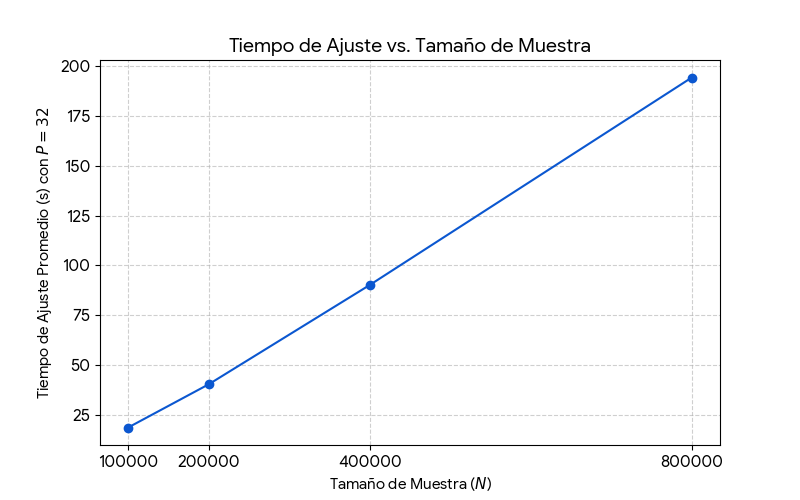
\includegraphics[width=0.8\textwidth]{fit_time_vs_n_jobs.png}
    \caption{Tiempo de Ajuste ($T_{\text{fit}}$) vs. Tamaño de Muestra ($N$) para $P=32$}
    \label{fig:fit_time_vs_n_samples_p32}
\end{figure}

La \textbf{Figura \ref{fig:fit_time_vs_n_samples_p32}} muestra cómo se comporta el tiempo de ajuste cuando el tamaño de la muestra ($N$) se incrementa, manteniendo el número de hilos constante en $P=32$.

\begin{itemize}
    \item \textbf{Escalamiento Super-Lineal}: Al aumentar $N$ por un factor de $8$ (de $100k$ a $800k$), el tiempo de ajuste se incrementa de $18.89s$ a $194.10s$, lo que representa un factor de aumento de $\approx 10.27$ veces.
    \item \textbf{Consistencia con la Complejidad}: Este aumento es mayor que el factor lineal ($8$) y es consistente con la complejidad teórica de los algoritmos de árbol de decisión (que forman la base de Random Forest), la cual a menudo es aproximadamente $O(N \cdot \log(N))$. Esto confirma que, incluso con un alto grado de paralelismo, el costo computacional del algoritmo está dominado por el tamaño de la entrada.
\end{itemize}

\section{Conclusiones}

El análisis de los resultados del experimento de Random Forest en el sistema HPC lleva a las siguientes conclusiones:

\begin{enumerate}
    \item \textbf{Efectividad del Paralelismo}: La paralelización del entrenamiento del Random Forest con \texttt{n\_jobs} es altamente efectiva para reducir el tiempo de ejecución, logrando una aceleración de $\approx 14.5$ para $P=32$ en el caso de $N=100k$.
    \item \textbf{Límites de Escalabilidad}: A partir de $P=16$, la ganancia de rendimiento por hilo adicional comienza a disminuir notablemente, indicando que se ha alcanzado el límite de escalabilidad para este tamaño de problema y configuración, donde la sobrecarga de paralelismo compensa las ganancias.
    \item \textbf{Impacto del Tamaño de la Muestra}: El tiempo de ajuste escala de manera super-lineal con el tamaño de la muestra ($N$), lo cual es el factor dominante en el costo computacional para grandes volúmenes de datos.
\end{enumerate}

Para futuras ejecuciones, se recomienda evaluar si el uso de más de 16 hilos proporciona un retorno de inversión en tiempo suficiente para justificar el uso de los recursos de cómputo, especialmente para los tamaños de muestra más pequeños.

\end{document}